\section{Cassandra Hardware Architecture}
\label{section_5}

% \subsection{Why New hardware?}
% Most commercial GPUs and NPUs do not support the majority of algorithms used in Cassandra, such as shared exponent, Huffman coding, and unstructured sparsity. Unless we redesign the compute cores, we must decode the encoded data from Cassandra and then perform computations using the existing floating-point units.

% Neither the MX format nor the Huffman coded exponent is natively supported by most current GPUs. Furthermore, while we employ bitmap-based unstructured sparsity, this method is not directly supported by the GPU's tensor cores. The critical issue is that these methods all involve bit-level operations or possess sequential decoding characteristics, which make the decoding process highly inefficient on SIMD-based xPUs. Consequently, we require a process to decode the data compressed in the Cassandra format back to the original tensor format before computation.

% For example, for Huffman coding decoding on a GPU, the fastest approach is to use a LUT-based decompression method. However, these methods demand a very large Shared memory area, and their speed is still far too slow for use in real-time LLM inference. In prior work, even with optimized custom CUDA kernels written for LLMs, these kernels could only achieve up to 50\% of the baseline performance when run on an actual GPU.
% Therefore, we propose a unified encoder and decoder to efficiently support the Cassandra algorithms, including the shared exponent. This unit can be efficiently applied to all Cassandra algorithms that utilize both Huffman and MX format. Additionally, it is highly area and power efficient as it does not require separate MAC logic. Because it operates separately from the compute units and memory, supporting a pipelined operation, its impact on throughput is also negligible. Our proposed Cassandra can be applied to various parallel processors, including GPUs and NPUs. Therefore, in the subsequent chapters, we will first describe the encoder and decoder architectures, and then present case studies for both the GPU and the NPU.


\subsection{Cassandra Encoder $\&$ Decoder Architecture}
\label{section_5_1}
To actually enhance the performance of xPU with Cassandra, low-overhead decompression is necessary. In contrast, operations such as MX format to floating point transformation, unary coding, and bitmap-based de-sparsification all require bit-level decoding computations. Performing these operations sequentially on a typical SIMD core cannot fully leverage hardware parallelism. Also, utilizing Cassandra necessitates online KV cache format conversion, and the operations used in this process, such as top-$k$ computations, can also be a potential burden. Therefore, we propose a Cassandra decoder and encoder to achieve high performance and low overhead format transformation, enabling the efficient use of Cassandra across various computing units.

 % Furthermore, even using parallel kernels for these tasks results in significant register overhead, leading to suboptimal decoding performance.

%%%%%%%%%%%%%%%%%%%%%%%%%%%%%%%%%%%%%%%%%%%%%%%%%%%%%%%%%%%%%%%%%%%%%%
\begin{figure}[t]
\centering
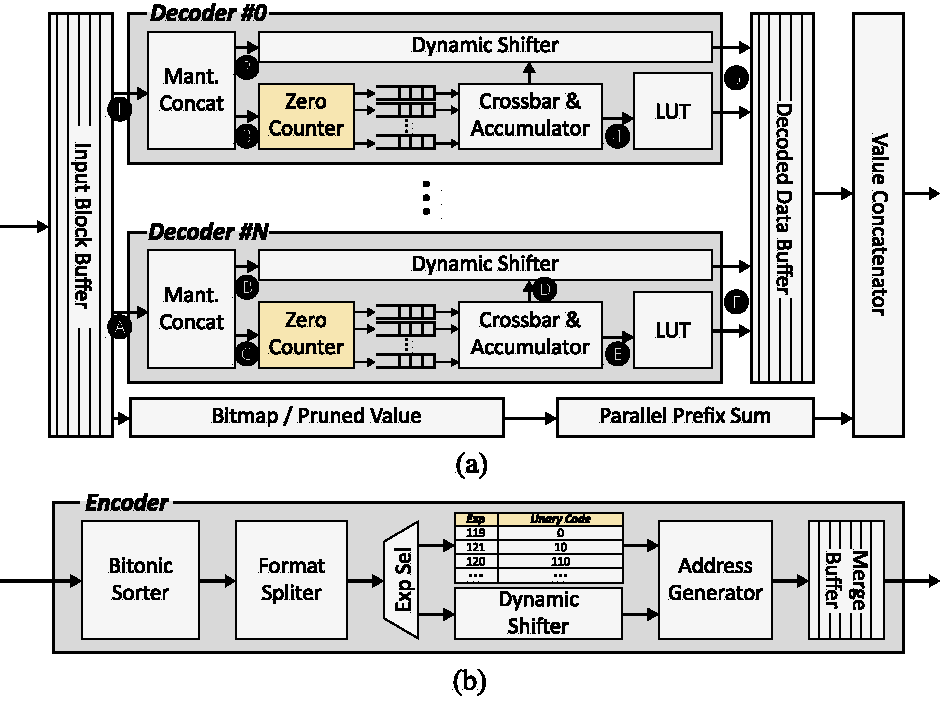
\includegraphics[width=\colimgwidth]{Figures/5_2_Encoder_Decoder.pdf}
\caption{(a) Microarchitecture and dataflow of Cassandra decoder. (b) Microarchitecture of Cassandra encoder.}
\label{fig_5_2}
\end{figure}
%%%%%%%%%%%%%%%%%%%%%%%%%%%%%%%%%%%%%%%%%%%%%%%%%%%%%%%%%%%%%%%%%%%%%%
%%%%%%%%%%%%%%%%%%%%%%%%%%%%%%%%%%%%%%%%%%%%%%%%%%%%%%%%%%%%%%%%%%%%%%
\begin{figure}[t]
\centering
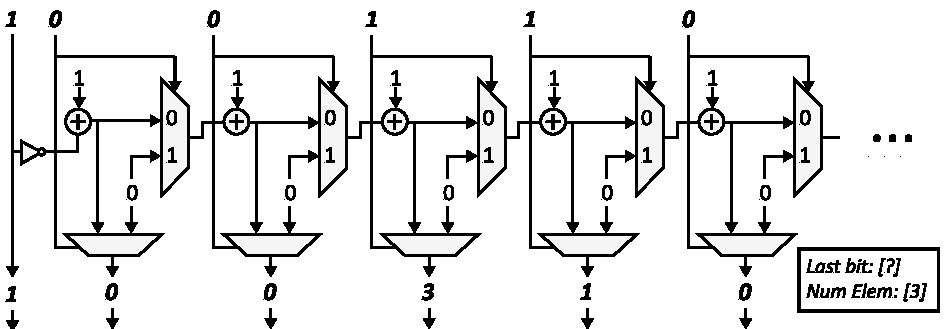
\includegraphics[width=\colimgwidth]{Figures/5_1_Parallel_Counter.pdf}
\caption{Microarchitecture of parallel zero counter.}
\label{fig_5_1}
\vspace{-1.5em}
\end{figure}
%%%%%%%%%%%%%%%%%%%%%%%%%%%%%%%%%%%%%%%%%%%%%%%%%%%%%%%%%%%%%%%%%%%%%%

Figure~\ref{fig_5_2} illustrates the architecture of our decoder and encoder, and how these hardware components operate across different dataflows. Decoder \#0 in Figure~\ref{fig_5_2}(a) demonstrates the decoding dataflow when using the unary coding for exponent compression. Initially, the low bits and high bits of the truncated mantissa are concatenated in the \myfilledcircled{1}~\textbf{mantissa concatenator}. Subsequently, the sign and mantissa are fed to the \myfilledcircled{2}~\textbf{dynamic shifter} and await exponent decoding. The exponent is uniformly sliced into 8-bit chunks and sent to the \myfilledcircled{3}~\textbf{parallel zero counter}.

Figure~\ref{fig_5_1} presents the microarchitecture of a parallel zero counter. For each bit position, the module outputs the cumulative number of preceding zeros up to that position. In parallel, it also produces the total count of input ones and the value of the final bit. The output from the parallel zero counter passes through a zero eliminator and enters a queue, where it is used as an index for the \myfilledcircled{4}~\textbf{LUT} for unary decoding. 

% Although we arbitrarily segmented the sequentially encoded exponents into 8-bit chunks and input them into a parallel zero counter, obtaining the correct decoding value necessitates information from the preceding bits. This can be resolved in each chunk by recalculating the value after receiving, in parallel, the last bit of the previous chunk and the count of consecutive zeros obtained from that preceding operation.

Although we arbitrarily segmented the sequentially encoded exponents into 8-bit chunks and input them into a parallel zero counter, obtaining the correct decoding value necessitates information from the preceding bits. This challenge can be addressed by recalculating in each chunk, which involves concurrently receiving the last bit of the preceding chunk and the count of consecutive zeros last obtained from that preceding chunk. Algorithm~\ref{algorithm_1} describes the entire process of exponent decoding within a parallel zero counter. After these processes, a \myfilledcircled{5}~\textbf{bitmap-based} de-sparsification operation is performed to derive the final output.

%%%%%%%%%%%%%%%%%%%%%%%%%%%%%%%%%%%%%%%%%%%%%%%%%%%%%%%%%%%%%%%%%%%%%%
\begin{algorithm}[t] % [H] 옵션은 알고리즘을 "여기(here)"에 위치시킴
\caption{Pseudo Code of Parallel Unary Decoding\label{alg:search}}
\label{algorithm_1}
% Input
\KwIn{N-bit unary coded exponent $U$, the number of element $numel$}
% Output
\KwOut{Set of decoded 8bit exponents $Exp$}

\tcc{Parallel Zero Counting}

$[Chunk_0, Chunk_1, ..., Chunk_{[\frac{N}{8}]}] \leftarrow \func{DevideInto8bitChunk}(U)$

$i,k,l, sum, idx \leftarrow 0$

\While{$i < [N//8] $}{
    $cnt\leftarrow 0$,
    $reorganized_i \leftarrow Chunk_i[7]$
    
    $num\_ones_i \leftarrow \func{NumberofOnes}(Chunk_i)$
    
    \For{$j$ in $range(8)$ } {
        \eIf{$Chunk_i[j]==0$}
        {
            % $output_{ij}\leftarrow 0$, \
            $cnt \leftarrow cnt + 1$
        }{
            $output_{i}.append(cnt)$, \
            $cnt\leftarrow 0$
        }
    }
    $i \leftarrow i+1$
}

\tcc{Parallel Reorganization}

\While{$k < [N//8] $}{
    \eIf{$reorganized_k==0$}
    {
        $sum \leftarrow sum + cnt_k$
    }{
        $output_{k}[0]\leftarrow output_{k}[0] + sum$ \\
        $sum \leftarrow 0$
    }
    $k \leftarrow k+1$
}

\While{$l < [N//8] $}{
    \For{$m \; in\;  range(num\_ones_{l}) $}{
    $Exp_{idx} \leftarrow \func{UnaryCodebook}(output_{l}[m])$
    $idx \leftarrow idx+1$ \\
    \If{$idx > numel$}{
    \KwRet{$Exp$}
    }
    }
}

\KwRet{$Exp$} % \KwRet은 "return" 키워드를 의미

\end{algorithm}
%%%%%%%%%%%%%%%%%%%%%%%%%%%%%%%%%%%%%%%%%%%%%%%%%%%%%%%%%%%%%%%%%%%%%%
% \vspace{-3em}
Decoder \#N in Figure~\ref{fig_5_2}(a) demonstrates the decoding dataflow when using the MX format. The low-bits and high-bits of the mantissa are combined by the \myfilledcircled{A}~\textbf{mantissa concatenator} first. However, in this case, after the mantissa is combined, the mantissa is fed into the input of both \myfilledcircled{B}~\textbf{dynamic shifter} and \myfilledcircled{C}~\textbf{parallel zero counter}. In this case, the exponent is first passed through a crossbar and broadcast to the accumulator corresponding to each element. Subsequently, the parallel zero counter counts the number of zeros in the mantissa, determining how many bits each mantissa should be shifted and how much should be subtracted from the exponent. Since it is guaranteed that one counter processes one mantissa, adjustment with adjacent chunks is not necessary. Once the shifted value for each mantissa is determined, this value is sent to the \myfilledcircled{D}~\textbf{dynamic shifter} to perform mantissa shifting and simultaneously subtracted from the exponent in the \myfilledcircled{E}~\textbf{accumulator}. Afterwards, the decoding process concludes by performing \myfilledcircled{F}~\textbf{bitmap-based} de-sparification, similar to Cassandra-1.

% Although this decoding process takes up to N cycles, during LLM inference, uninterrupted memory loads occur, and the hardware operates in a pipelined manner between these loads, which significantly hides the latency overhead.

The operation of the Cassandra encoder is comparatively simpler. When data is first input, the encoder finds the top-$k$ values in this data and divides them into a speculation group and a verification group. The verification group is stored in a buffer immediately, along with a bitmap, without any further transformation. The data belonging to the speculation group undergoes different exponent compression processes depending on whether they use MX format or unary coding, followed by mantissa truncation, and then they are stored in the buffer. Subsequently, the values stored in the buffer are saved to main memory. Since weights can be formatted offline before storage, this encoder is primarily used for online formatting of the KV cache.



\subsection{Integrating Cassandra with xPU}
\label{section_5_2}
\begin{figure*}[t!]
\centering
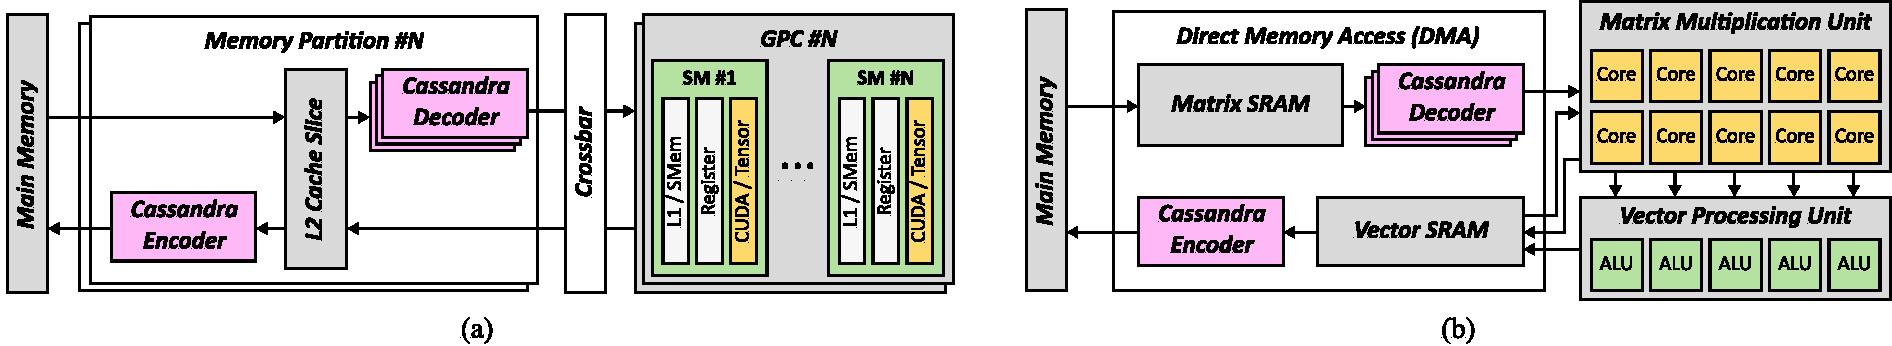
\includegraphics[width=\fullimgwidth]{Figures/5_2_Cassandra_Integration.pdf}
\caption{Overall architecture of (a) Cassandra-integrated GPU and (b) Cassandra-integrated systolic array based NPU}
\label{fig_5_3}
\end{figure*}

Cassandra is designed to operate alongside the memory system of a GPU and NPU. A GPU utilizes a partitioned memory system architecture, where each memory channel has its own dedicated L2 cache slice and memory controller. Furthermore, all data originating from the main memory must pass through the L2 cache before being delivered to the L1 cache or shared memory. Figure~\ref{fig_5_3}(a) illustrates how Cassandra can be integrated into such a system. Because sharing data between memory partitions is challenging in a GPU, Cassandra encoder and decoder should be installed independently for each memory partition.
In this configuration, the decoder is placed between the L2 cache and the interconnect, and the encoder is situated between the main memory and the L2 cache. This placement allows for the efficient utilization of both memory bandwidth and L2 cache capacity and bandwidth. In this case, Cassandra's encoder and decoder are managed by the memory controller, similar to the L2 cache.

To distinguish standard data types (e.g., activations) from specially formatted weights and KV cache, the user must explicitly specify the data type being stored (i.e., floating-point or Cassandra format) during the memory allocation process. Data of the standard datatype and the Cassandra datatype are then stored in separate virtual pages. To distinguish the data type held by each page, the page table and TLBs must be provisioned with spare bits. Since commercial GPUs from vendors like Nvidia and AMD already include spare bits in their page table entries, this modification introduces no additional overhead.~\cite{ecco}.

For an NPU with a DMA-based memory system, as shown in Figure~\ref{fig_5_3}(b), it is reasonable to place both the encoder and decoder within the DMA. This structure is similar to the one in GPUs, but in this case, the encoder and decoder should be managed by the DMA controller. Also, unlike GPUs, many NPUs do not use a virtual memory system. Therefore, in this scenario, the physical memory addresses for storing the standard datatypes and Cassandra datatypes must be separated, and this information must be pre-stored in the DMA controller to ensure appropriate encoding and decoding.

Decoding overhead in Cassandra can slow down the read speed of weights and the KV cache, degrading overall system performance, while the encoder's performance is irrelevant to this. Hence, the decoder should be sufficiently added to match the maximum throughput of the L2 cache, while a comparatively smaller number of encoders may be sufficient.

\subsection{Superblock based Data Management}
Variable sequence length in unary encoding, as well as the potential difference in the ratio between speculation data and verification data that may arise when sparsity changes, makes memory mapping more challenging. Specifically, in a cache-based memory system like a GPU, this difficulty in mapping data to perfectly fit a cache block can lead to performance degradation due to redundant data loads. To eliminate this potential performance bottleneck, we propose a superblock-based memory mapping scheme. For a cache-based system, Cassandra sets a group of multiple cache blocks, which we refer to as a superblock, as the fundamental unit for load and eviction. This superblock is fully packed with cache blocks containing various data types, such as bitmaps, variable exponents, and mantissas. Initially, when data is loaded, the entire superblock is loaded at once and stored in the L2 cache. These data are subsequently fed into the decoder.

%%%%%%%%%%%%%%%%%%%%%%%%%%%%%%%%%%%%%%%%%%%%%%%%%%%%%%%%%%%%%%%%%%%%%%
\label{section_5_3}
\begin{figure}[t]
\centering
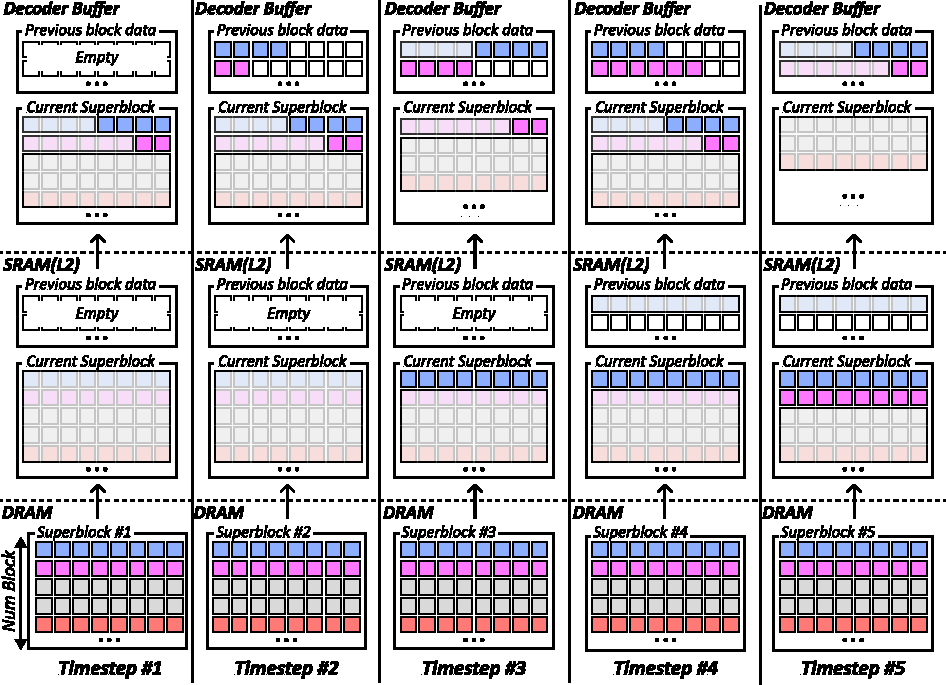
\includegraphics[width=\colimgwidth]{Figures/5_3_Superblock.pdf}
\caption{Visualization of superblock-based data management.}
\label{fig_5_4}
\vspace{-1.0em}
\end{figure}
%%%%%%%%%%%%%%%%%%%%%%%%%%%%%%%%%%%%%%%%%%%%%%%%%%%%%%%%%%%%%%%%%%%%%%

During the decoding process, depending on the sparse ratio or the length of the exponent, some data types might not fully utilize all the data contained within a single cache block, resulting in leftover data. The decoder stores this leftover data in its internal buffer and concatenates it with the data from the next cache block of that type when it is read.

If the size of the data in the decoder buffer exceeds 128 bytes, the memory controller skips sending the corresponding type of cache block to the decoder. It also keeps track of how many times the block of that type has been skipped for the next read. In this manner, the memory controller manages the address values of each type of cache block that should be fed into the decoder next, sending them to the decoder as needed.

This approach guarantees contiguous data reads from global memory and dense memory mapping, preventing potential degradation in memory performance. This method also works efficiently in scratchpad-based devices, such as NPUs, where issues like row buffer misses and page misses can still occur. For an NPU, the same mechanism can be applied by directly setting an arbitrary block size, rather than a cache block size.